\documentclass[10pt,a4paper]{article}
\usepackage[latin1]{inputenc}
\usepackage[spanish]{babel}
\usepackage{amsmath}
\usepackage{amsfonts}
\usepackage{amssymb}
\usepackage{graphicx}
\usepackage[left=2cm,right=2cm,top=2cm,bottom=2cm]{geometry}
\author{Jorge Marroqu�n}
\begin{document}

\begin{flushleft}
\textbf{Nombre: }Jorge Armando Marroqu�n Ochoa
\end{flushleft}
\textbf{Carnet: }2018358\\

\begin{center}
        \huge{Hoja de trabajo \#1} \\
\end{center}

\section{Ejercicio \#2} 
\begin{center}
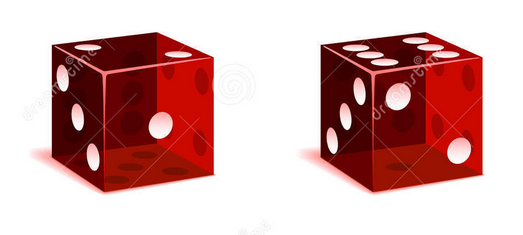
\includegraphics[width=9cm]{dado.png}
\end{center}
\begin{enumerate}
\item {$\{1,2,3,4,5,6\}$}
\item {
\begin{tabular}{p{0cm} c}
    $$
    \left\{
        \begin{bmatrix}
            \langle 1,2 \rangle & \langle 1,3 \rangle & \langle 1,4 \rangle & \langle 1,5 \rangle \\
            \langle 2,1 \rangle & \langle 2,3 \rangle & \langle 2,4 \rangle & \langle 2,6 \rangle \\
            \langle 3,1 \rangle & \langle 3,2 \rangle & \langle 3,5 \rangle & \langle 3,6 \rangle \\
            \langle 4,1 \rangle & \langle 4,2 \rangle & \langle 4,5 \rangle & \langle 4,6 \rangle \\
            \langle 5,1 \rangle & \langle 5,3 \rangle & \langle 5,4 \rangle & \langle 5,6 \rangle \\
            \langle 6,2 \rangle & \langle 6,3 \rangle & \langle 6,4 \rangle & \langle 6,5 \rangle \\
        \end{bmatrix}
    \right\}
$$

\end{tabular}
}
\end{enumerate}

\section{Ejercicio \#3}
\begin{enumerate}
\item {\textbf{�Que estructura de datos podria representar un lanzamiento de dados?}}\\
Se puede representar como una estructura de camino.
\item {\textbf{�Que algoritmo podriamos utilizar para generar dicha estructura?}}\\
Es un algoritmo de camino para que puede llegar a un n�mero.
\item {\textbf{�Como nos aseguramos que ese algoritmo siempre produce un resultado?}}\\
El algoritmo debe segir un camino l�gico, si pasa de un n�mero cualquiera a su cara opuesta, este no sirve porque no pasa por un camino l�gico.
\end{enumerate}
\end{document}